TABLES
\setlength\parindent{24pt}
        \begin{table}[h!]
        \centering
        \begin{tabular}{|c|c|c|}
        \hline
        Node & Ex. & Categories\\
        \hline
        1. & 23105 & apparel, office products, automotive, toys games, \\ 
        & &  computer video games, software\\
        2. & 18146 & grocery, beauty, magazines, jewelry watches, \\
        & & sports outdoors, cell phones service, baby\\
        3. & 54333 & outdoor living, video, camera photo, \\
        & & health personal care, gourmet food, music\\
        \textit{Test} & \textit{21064} & \textit{books, dvd, electronics, kitchen housewares}\\
        \hline
        \end{tabular}
        \caption{Portions of the dataset assigned to each node in the IN experiments.}\label{tab:cats_in}
        \end{table}




        \begin{table}[h!]
        \centering
        \begin{tabular}{|c|c|c|}
        \hline
        Node & Ex. & Categories\\
        \hline
        1. & 30 & books\\
        2. & 30 & dvd\\
        3. & 30 & electronics\\
        4. & 30 & kitchen housewares\\
        \textit{Test} & \textit{21064} & \textit{books, dvd, electronics, kitchen housewares}\\
        \hline
        \end{tabular}
        \caption{Portions of the dataset assigned to each node in the BART experiments.}\label{tab:cats_b}
        \end{table}
        

        \begin{table}[h!]
      \centering
      \begin{tabular}{|c|c|}
        \hline
        Model & Mean Accuracy (\%) \\
        \hline
        Node 1 & 83.5 \\
        Node 2 & 83.3 \\
        Node 3 & 83.1 \\
        Averaging & 84.6 \\
        Stacking & 84.6 \\
        Reproduced model from \cite{geng2019induction} & 83.9 \\
        Result reported in \cite{geng2019induction} (SoTA) & 85.6 \\
        \hline
      \end{tabular}
      \caption{Results obtained with Induction Network from \cite{geng2019induction}.}\label{Tab:induction_results}
    \end{table}
    
    Table \ref{Tab:bart_results} shows the results obtained with the BART model (with and without fine-tuning). The values between parentheses give the standard deviation of the results after 5 trials.
    
    TODO: report statistical confidence interval at 90\% (look for Wald test):
    $$\pm 1.96 \sqrt{\frac {p(1-p)}{n=9000}}$$
    

    \begin{table}[h!]
      \centering
      \hspace*{-40pt}\begin{tabular}{|c|c|c|c|c|c|}
        \hline
        Model & MA & Books & DVD & Electronics & KH \\
        \hline
        ZSL & 83.0 & 82.7 & 80.2 & 84.3 & 84.8 \\
        Books Node & 85.1[$\pm 0.23$] & 86.4[$\pm 0.2$] & 83.4[$\pm 0.29$] & 85.0[$\pm 0.23$] & 85.3[$\pm 0.33]$ \\
        Dvd Node & 85.2[$\pm 0.11$] & 86.8[$\pm 0.1$] & 83.9[$\pm 0.34$] & 85.0[$\pm 0.22$] & 85.5[$\pm 0.29$]  \\
        Electronics Node & 84.4[$\pm 0.39$] & 84.4[$\pm 0.87$] & 82.1[$\pm 0.68$] & 85.3[$\pm 0.23$] & 86.1[$\pm 0.15$] \\
        Kitchen H. Node & 85.6[$\pm 0.12$] & 86.5[$\pm 0.22$] & 84.8[$\pm 0.37$] & 85.2[$\pm 0.22$] & 86.2[$\pm 0.17$]  \\
        Stacking & - & - & - & - & - \\ 
        Avg of 4 nodes & 85.9 & 81.5 & 84.6 & 86.2 & 85.9  \\
        Weighted Avg & 85.8 & 86.8 & 84.4 & 86.0 & 86.1  \\
        Federated Avg & 85.7 & 86.7 & 84.4 & 85.7 & 86.0  \\
        Model from \cite{geng-etal-2019-induction}\footnote{The model was reproduced.} & 83.9 & & & & \\
        SoTA Result \cite{geng-etal-2019-induction} & 85.6 & & & & \\
        \hline
      \end{tabular}
      \caption{Results obtained with BART.}\label{Tab:bart_results}
    \end{table}


INTRO

Google's T5 model, which is designed to perform well on data-scarce tasks. The results of a few experiments are reported, together with a brief summary of our findings.

%To overcome this problem, the few-shot learning methods could be used \cite{wang2020generalizing}. The algorithms based on this method may be easily applied to the new previously unseen classes with only a few training samples. Thus, a federated model could be retrained for a new user with only a few examples. Nevertheless, these models require a huge dataset during the prior training, so one of the crucial federated learning limitations is still present.

% I don't know how to express in a nice way the idea about the prior training that is needed. the process of training a FS model starts with the big dataset that has a lot of examples of, for example, 4 classes (each of them has a loooot of examples). then, after the training it is believed that we no longer need a big dataset for new classes, just 5 examples. so we give these 5 new examples for the new class and it starts predicting them correctly. this is the idea....

%In this paper we propose a solution to each of these problems. We report the results of the experiments with the BART model that does not require a big manually annotated dataset and may be trained for a new task only on a few examples


FS
\subsection{Few-shot learning}
            Few-shot learning is a machine learning method used to generalise to a new task based on prior knowledge of other tasks \cite{wang2020generalizing}. It is mainly used when data for a specific task is scarce.
            
            A common way to approach few-shot learning consists in meta-learning a model to mimic few-shot learning scenarios. This is achieved through an episode-based training procedure \cite{NIPS2016_90e13578}. 
            
            For the task of few-shot text classification, \cite{geng2019induction} proposed the use of Induction Networks. An Induction Network is a Deep Learning architecture composed of a novel induction module that implements what is called a Dynamic Routing algorithm. This module enables the learning of generalized class representations, as opposed to static class representations that fail to generalize beyond training data.
            



METHOD
on two federated datasets for sentiment analysis. The first, Amazon Review \cite{yu2018diverse} has proven to perform well with few-shot learning and will be separated into nodes which each represent a device in a federated setting. The second, Sent140 \cite{caldas2019leaf}, is a federated dataset composed of Twitter comments, where each user corresponds to a node. We will use an Induction Network, which leverages meta-learning to carry out classification tasks.

Google's T5 model, which is designed to perform well on tasks for which data is particularly scarce. Our results will then be compared with the current benchmark for each dataset \textcolor{green}{\textbf{\cite{Bench1}}} \textcolor{green}{\textbf{\cite{Bench2}}}

    %\subsection{Induction Networks}
    %An Induction Network \cite{geng2019induction} is composed of three modules. The fist one is an encoder consisting of a bidirectional RNN with self attention. The second is an induction layer which enables the learning of generalized class representations.



DS
Sent140 \cite{caldas2019leaf} is a federated dataset whose tweets are automatically annotated based on the emoticons present in them. Each device is represented by a different twitter user.




            \subsection{Text-To-Text Transfer Transformer}
            Text-To-Text Transfer Transformer (T5) \cite{t5} is a language model with a text-to-text framework where the input consists in the description of the task and the data on which the task is to be carried out.
            
            \begin{figure}[h]
            \begin{center}
            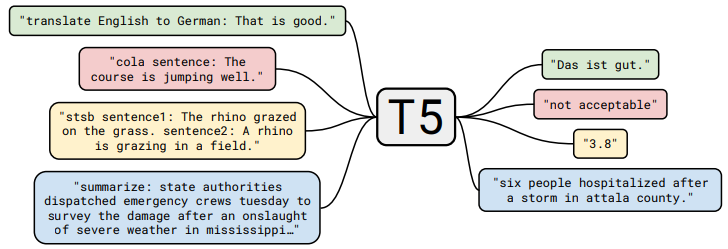
\includegraphics[width=\textwidth]{pics/T5.png}
            \caption{T5 input and output examples, as illustrated in the original paper \cite{t5}.}
            \label{fig:user}
            \end{center}
            \end{figure}
          
EXPERIMENTS
As the dataset contains 23 topics in total, 4 of which are reserved as a test set, we divided the remaining 19 topics into 3 groups which were used as separate nodes for training of the Induction model. The division has been done in the following way:
    \begin{itemize}
        \item First node (6 domains) - apparel, office products, automotive, toys games, computer video games, software;
        \item Second node (7 domains) - grocery, beauty, magazines, jewelry watches, sports outdoors, cell phones service, baby\footnote{"baby" domain was excluded from this node for testing the stacking approach};
        \item Third node (6 domains) - outdoor living, video, camera photo, health personal care, gourmet food, music.
    \end{itemize}
